% Options for packages loaded elsewhere
\PassOptionsToPackage{unicode}{hyperref}
\PassOptionsToPackage{hyphens}{url}
%
\documentclass[
  10pt,
  ignorenonframetext,
]{beamer}
\usepackage{pgfpages}
\setbeamertemplate{caption}[numbered]
\setbeamertemplate{caption label separator}{: }
\setbeamercolor{caption name}{fg=normal text.fg}
\beamertemplatenavigationsymbolsempty
% Prevent slide breaks in the middle of a paragraph
\widowpenalties 1 10000
\raggedbottom
\setbeamertemplate{part page}{
  \centering
  \begin{beamercolorbox}[sep=16pt,center]{part title}
    \usebeamerfont{part title}\insertpart\par
  \end{beamercolorbox}
}
\setbeamertemplate{section page}{
  \centering
  \begin{beamercolorbox}[sep=12pt,center]{part title}
    \usebeamerfont{section title}\insertsection\par
  \end{beamercolorbox}
}
\setbeamertemplate{subsection page}{
  \centering
  \begin{beamercolorbox}[sep=8pt,center]{part title}
    \usebeamerfont{subsection title}\insertsubsection\par
  \end{beamercolorbox}
}
\AtBeginPart{
  \frame{\partpage}
}
\AtBeginSection{
  \ifbibliography
  \else
    \frame{\sectionpage}
  \fi
}
\AtBeginSubsection{
  \frame{\subsectionpage}
}
\usepackage{amsmath,amssymb}
\usepackage{lmodern}
\usepackage{iftex}
\ifPDFTeX
  \usepackage[T1]{fontenc}
  \usepackage[utf8]{inputenc}
  \usepackage{textcomp} % provide euro and other symbols
\else % if luatex or xetex
  \usepackage{unicode-math}
  \defaultfontfeatures{Scale=MatchLowercase}
  \defaultfontfeatures[\rmfamily]{Ligatures=TeX,Scale=1}
\fi
% Use upquote if available, for straight quotes in verbatim environments
\IfFileExists{upquote.sty}{\usepackage{upquote}}{}
\IfFileExists{microtype.sty}{% use microtype if available
  \usepackage[]{microtype}
  \UseMicrotypeSet[protrusion]{basicmath} % disable protrusion for tt fonts
}{}
\makeatletter
\@ifundefined{KOMAClassName}{% if non-KOMA class
  \IfFileExists{parskip.sty}{%
    \usepackage{parskip}
  }{% else
    \setlength{\parindent}{0pt}
    \setlength{\parskip}{6pt plus 2pt minus 1pt}}
}{% if KOMA class
  \KOMAoptions{parskip=half}}
\makeatother
\usepackage{xcolor}
\IfFileExists{xurl.sty}{\usepackage{xurl}}{} % add URL line breaks if available
\IfFileExists{bookmark.sty}{\usepackage{bookmark}}{\usepackage{hyperref}}
\hypersetup{
  pdftitle={Screening Designs},
  pdfauthor={BIOE 498/598 PJ},
  hidelinks,
  pdfcreator={LaTeX via pandoc}}
\urlstyle{same} % disable monospaced font for URLs
\newif\ifbibliography
\usepackage{graphicx}
\makeatletter
\def\maxwidth{\ifdim\Gin@nat@width>\linewidth\linewidth\else\Gin@nat@width\fi}
\def\maxheight{\ifdim\Gin@nat@height>\textheight\textheight\else\Gin@nat@height\fi}
\makeatother
% Scale images if necessary, so that they will not overflow the page
% margins by default, and it is still possible to overwrite the defaults
% using explicit options in \includegraphics[width, height, ...]{}
\setkeys{Gin}{width=\maxwidth,height=\maxheight,keepaspectratio}
% Set default figure placement to htbp
\makeatletter
\def\fps@figure{htbp}
\makeatother
\setlength{\emergencystretch}{3em} % prevent overfull lines
\providecommand{\tightlist}{%
  \setlength{\itemsep}{0pt}\setlength{\parskip}{0pt}}
\setcounter{secnumdepth}{-\maxdimen} % remove section numbering
\ifLuaTeX
  \usepackage{selnolig}  % disable illegal ligatures
\fi

\title{Screening Designs}
\author{BIOE 498/598 PJ}
\date{Spring 2022}

\begin{document}
\frame{\titlepage}

\begin{frame}{Why do we use screening designs?}
\protect\hypertarget{why-do-we-use-screening-designs}{}
\newcommand\lo{\ensuremath{\boldsymbol{-}}}
\newcommand\hi{\ensuremath{\boldsymbol{+}}}
\newcommand\iii{\ensuremath{\mathrm{III}}}
\newcommand\iv{\ensuremath{\mathrm{IV}}}
\newcommand\vv{\ensuremath{\mathrm{V}}}

\begin{itemize}
\tightlist
\item
  Optimization is expensive---many runs/factor at \(>2\) levels
\item
  Too many factors wastes resources
\item
  Too few factors leads to suboptimal results
\end{itemize}

\pause

\begin{itemize}
\tightlist
\item
  \textbf{Solution:} A \emph{screening design} tests a large number of
  factors
\item
  Only active factors are carried forward for optimization
\end{itemize}
\end{frame}

\begin{frame}{What is a screening design?}
\protect\hypertarget{what-is-a-screening-design}{}
\begin{itemize}
\tightlist
\item
  Screening designs have few runs, ideally \(\le 2\) runs/factor. \pause
\item
  The focus is on main effects. By the Effect Hierarchy and Effect
  Heredity principles,
  \[ \text{important factor} \approx \text{significant main effect} \]
\end{itemize}

\pause

\begin{itemize}
\tightlist
\item
  We don't worry about estimates of TWIs. We're selecting factors, not
  interactions.
\end{itemize}
\end{frame}

\begin{frame}{Types of screening designs}
\protect\hypertarget{types-of-screening-designs}{}
\begin{itemize}
\tightlist
\item
  Resolution \ensuremath{\mathrm{III}}~Fractional Factorial Design

  \begin{itemize}
  \tightlist
  \item
    Pro: Mirror image can clear main effects
  \item
    Con: Run size always a power of 2
  \end{itemize}
\end{itemize}

\pause

\begin{itemize}
\tightlist
\item
  PB Design

  \begin{itemize}
  \tightlist
  \item
    Pro: Run size in multiples of 4
  \item
    Con: Complex aliasing
  \end{itemize}
\end{itemize}

\pause

\begin{itemize}
\tightlist
\item
  Definitive Screening Designs

  \begin{itemize}
  \tightlist
  \item
    Hybrid screening/optimization design. We'll discuss later!
  \end{itemize}
\end{itemize}
\end{frame}

\begin{frame}{Don't rule out Fractional Factorial Designs.}
\protect\hypertarget{dont-rule-out-fractional-factorial-designs.}{}
\begin{center}\includegraphics[width=0.75\linewidth]{13_ScreeningDesigns_files/figure-beamer/unnamed-chunk-2-1} \end{center}
\end{frame}

\begin{frame}{Workflow for Resolution \ensuremath{\mathrm{III}}~screens}
\protect\hypertarget{workflow-for-resolution-screens}{}
\begin{enumerate}
\tightlist
\item
  Run the design
\item
  Fit the model with main effects. If you have DoF left over, add any
  TWIs that are \textbf{not} confounded with main effects.
\item
  If the overall model fit is bad, or if you expected certain effects to
  be significant that were not, consider a second batch of runs with a
  mirror image design.
\item
  Drop any factors that are not \textbf{important} (practically or
  statistically).
\end{enumerate}
\end{frame}

\begin{frame}{}
\protect\hypertarget{section}{}
\begin{columns}

\begin{column}{0.8\textwidth}
\begin{center}
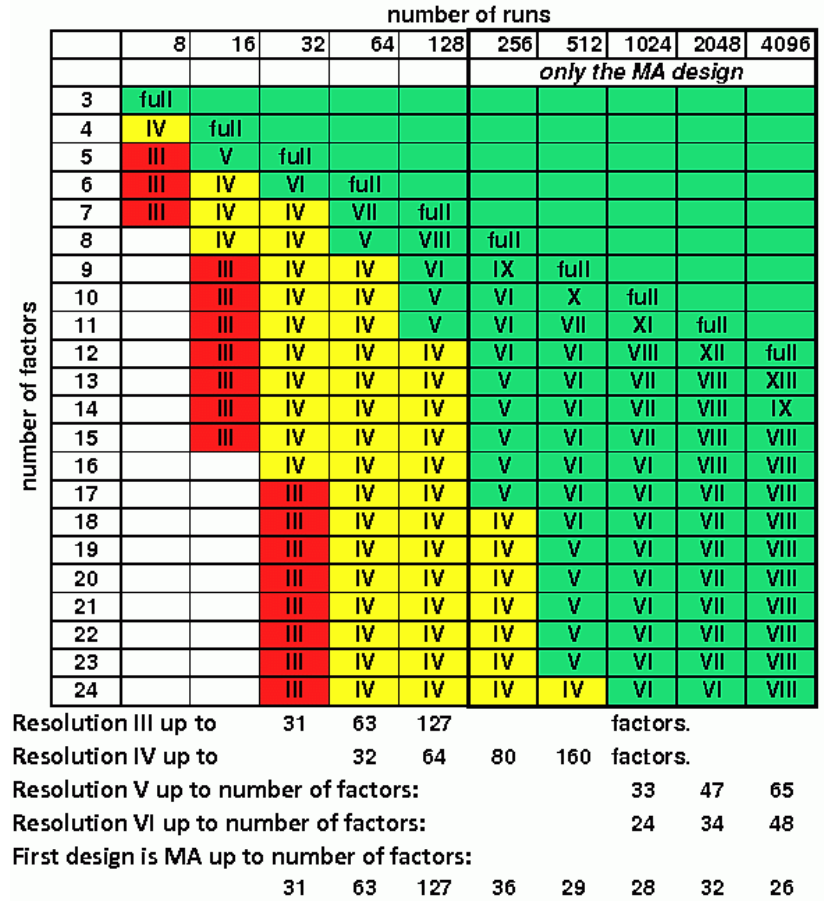
\includegraphics[width=\textwidth]{frf2-resolution.png}
\end{center}
\end{column}

\begin{column}{0.2\textwidth}
{\footnotesize Gromping, 2014\\ \emph{J.\ Stat.\ Software}}
\end{column}

\end{columns}
\end{frame}

\begin{frame}{Workflow for PB designs}
\protect\hypertarget{workflow-for-pb-designs}{}
\begin{enumerate}
\tightlist
\item
  Run the design.
\item
  Fit a model with main effects plus an effect for any unused column in
  the design.
\item
  Optional: Perform subset regression to identify factors that appear
  frequently in smaller models with good predictive power.
\item
  Drop any factors that are not \textbf{important} (practically or
  statistically).
\item
  If only a small number of factors remain, try refitting the small
  model.
\end{enumerate}
\end{frame}

\begin{frame}{Creating a PB design (up to 23 factors)}
\protect\hypertarget{creating-a-pb-design-up-to-23-factors}{}
\begin{enumerate}
\tightlist
\item
  Start with the first run from the following table.
\end{enumerate}

\medskip
\begin{center}
\begin{tabular}{cl}
Runs & Factor Levels \\
\hline
12 & \ensuremath{\boldsymbol{+}}\,\ensuremath{\boldsymbol{+}}\,\ensuremath{\boldsymbol{-}}\,\ensuremath{\boldsymbol{+}}\,\ensuremath{\boldsymbol{+}}\,\ensuremath{\boldsymbol{+}}\,\ensuremath{\boldsymbol{-}}\,\ensuremath{\boldsymbol{-}}\,\ensuremath{\boldsymbol{-}}\,\ensuremath{\boldsymbol{+}}\,\ensuremath{\boldsymbol{-}}\\
20 & \ensuremath{\boldsymbol{+}}\,\ensuremath{\boldsymbol{+}}\,\ensuremath{\boldsymbol{-}}\,\ensuremath{\boldsymbol{-}}\,\ensuremath{\boldsymbol{+}}\,\ensuremath{\boldsymbol{+}}\,\ensuremath{\boldsymbol{+}}\,\ensuremath{\boldsymbol{+}}\,\ensuremath{\boldsymbol{-}}\,\ensuremath{\boldsymbol{+}}\,\ensuremath{\boldsymbol{-}}\,\ensuremath{\boldsymbol{+}}\,\ensuremath{\boldsymbol{-}}\,\ensuremath{\boldsymbol{-}}\,\ensuremath{\boldsymbol{-}}\,\ensuremath{\boldsymbol{-}}\,\ensuremath{\boldsymbol{+}}\,\ensuremath{\boldsymbol{+}}\,\ensuremath{\boldsymbol{-}}\\
24 & \ensuremath{\boldsymbol{+}}\,\ensuremath{\boldsymbol{+}}\,\ensuremath{\boldsymbol{+}}\,\ensuremath{\boldsymbol{+}}\,\ensuremath{\boldsymbol{+}}\,\ensuremath{\boldsymbol{-}}\,\ensuremath{\boldsymbol{+}}\,\ensuremath{\boldsymbol{-}}\,\ensuremath{\boldsymbol{+}}\,\ensuremath{\boldsymbol{+}}\,\ensuremath{\boldsymbol{-}}\,\ensuremath{\boldsymbol{-}}\,\ensuremath{\boldsymbol{+}}\,\ensuremath{\boldsymbol{+}}\,\ensuremath{\boldsymbol{-}}\,\ensuremath{\boldsymbol{-}}\,\ensuremath{\boldsymbol{+}}\,\ensuremath{\boldsymbol{-}}\,\ensuremath{\boldsymbol{+}}\,\ensuremath{\boldsymbol{-}}\,\ensuremath{\boldsymbol{-}}\,\ensuremath{\boldsymbol{-}}\,\ensuremath{\boldsymbol{-}}
\end{tabular}
\end{center}
\medskip

\begin{enumerate}
\setcounter{enumi}{1}
\item
  Cycle the factor levels by one to get run \#2. Repeat for 11, 19, or
  23 runs.
\item
  Set the final run to all low (\ensuremath{\boldsymbol{-}}).
\item
  If the number of factors \(k\) is less than the number of runs, select
  the first \(k\) columns.
\end{enumerate}
\end{frame}

\begin{frame}{Example PB design: Cast fatigue}
\protect\hypertarget{example-pb-design-cast-fatigue}{}
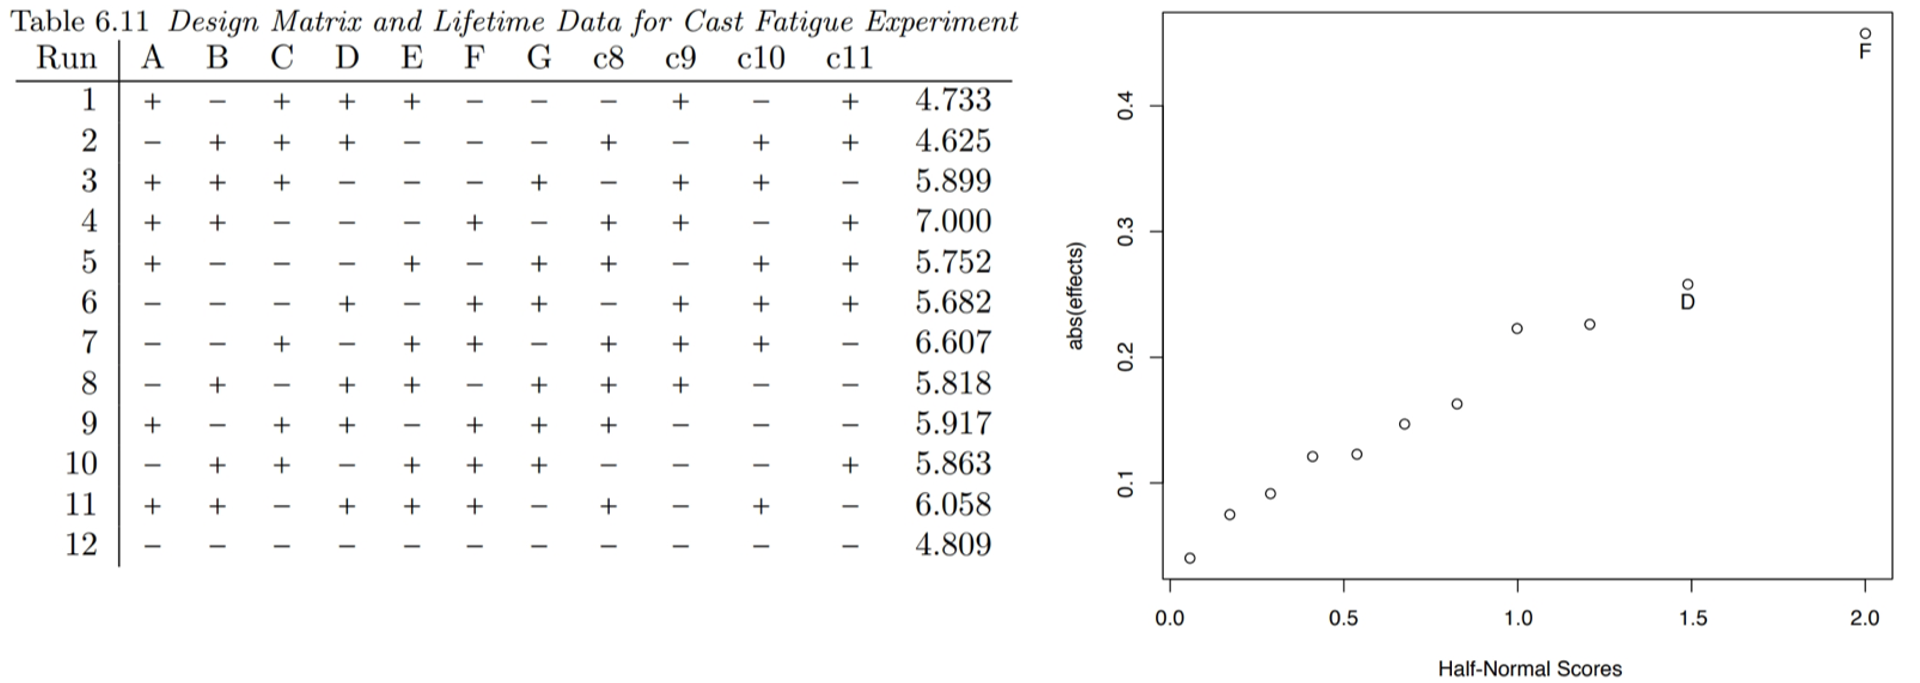
\includegraphics{figures/altfact2.png}

This design includes 7 factors; however, effects are estimated for all
columns. The last 4 ``factors'\,' are interactions with complex
aliasing.
\end{frame}

\begin{frame}{To replicate or not to replicate?}
\protect\hypertarget{to-replicate-or-not-to-replicate}{}
\begin{itemize}
\tightlist
\item
  Many screening designs are saturated --- there are no DoF to estimate
  confidence intervals for the parameters.
\item
  If you don't replicate the design, you will need to select factors
  based on the magnitude of the effects alone (half-normal plot).

  \begin{itemize}
  \tightlist
  \item
    Remember that half-normal plots work better as the number of factors
    grows.
  \end{itemize}
\end{itemize}

\pause

\begin{itemize}
\tightlist
\item
  Replicating a Resolution \ensuremath{\mathrm{III}}~Design

  \begin{itemize}
  \tightlist
  \item
    Consider a mirror-image instead. This will give clear main effects.
  \item
    Check if you can afford a Resolution
    \ensuremath{\mathrm{IV}}~instead. This gives clear main effects and
    a confounding structure.
  \end{itemize}
\item
  Replicating a PB Design

  \begin{itemize}
  \tightlist
  \item
    Replicating the design will help you estimate the ``pure error'\,'.
  \item
    You can ``move up'\,' to a larger PB design to get extra runs. This
    won't estimate pure error, but you can add more confounded effects
    to the model to improve the estimates.
  \end{itemize}
\end{itemize}
\end{frame}

\begin{frame}{Planning sequential experimentation}
\protect\hypertarget{planning-sequential-experimentation}{}
\begin{itemize}
\tightlist
\item
  This is difficult. Very, very difficult. There is no simple answer.
\end{itemize}

\pause

\begin{itemize}
\tightlist
\item
  The follow-up experiment is at higher resolution, so more runs/factor.
\item
  The follow-up experiment will also have fewer factors.
\end{itemize}

\pause

\begin{itemize}
\tightlist
\item
  Do a ``what-if'\,' analysis using varying numbers of dropped factors.
\item
  Replicates might be more important for a follow-up design.
\end{itemize}

\pause

\begin{itemize}
\tightlist
\item
  Where do you want the bottleneck?

  \begin{itemize}
  \tightlist
  \item
    Stringent screening (expensive) \(\rightarrow\) smaller follow-up
    (cheaper)
  \item
    Relaxed screening (cheaper) \(\rightarrow\) larger follow-up
    (expensive)
  \end{itemize}
\end{itemize}

\pause

\begin{itemize}
\tightlist
\item
  Use your experience in science or engineering. How much of your budget
  did you spend

  \begin{itemize}
  \tightlist
  \item
    Screening for a hit or working up the mechanism?
  \item
    Building/testing a prototype or refining the second design?
  \end{itemize}
\end{itemize}
\end{frame}

\begin{frame}{About grading}
\protect\hypertarget{about-grading}{}
\begin{itemize}
\tightlist
\item
  Your grade is determined by your process.
\item
  If your methods are justified and implemented correctly, you can earn
  full credit.
\item
  How your make your final predictions will be graded.
\item
  The result of your final predictions determines a few bonus points and
  bragging rights.
\end{itemize}
\end{frame}

\end{document}
